\chapter{Interpretation}\label{Kapitel 4}

% TODO Einleitung

\section{Linpack}\label{Interpretation Linpack}

\section{Whetstone}\label{Interpretation Whetstone}

\section{Einordnung in TOP500 und Green500}\label{Rankings}

% TODO TOP500 Einordnung

% Seit einigen Jahren zeigt sich auch in der HPC-Welt ein zunehmendes Problembewusstsein betreffend den Energieverbrauch und -effizienz der verwendeten und untersuchten Systeme. Daraus resultiert das Green500-Ranking, das seit dem Jahr 2006 die Kandidaten der TOP500-Liste unter dem Aspekt der Energieeffizienz untersucht. Die Bestenliste liefert die Supercomputer mit dem besten Verh"altnis zwischen Leistung und Stromverbrauch (FLOPS pro Watt)\footnote{Vgl. \url{http://www.green500.org/}.}.

% TODO Kriterien ausarbeiten
% Quelle: \url{http://www.green500.org/docs/pubs/RunRules_Ver1.0.pdf}

\endinput 

%Grafik aus PNG-File - bei dieser Variante darauf achten, dass die Grafik in ausreichender Auflösung vorliegt (so dass auch nach Skalierung >300dpi im Ausdruck erreicht werden) 
%\begin{figure}[htb]
%  \centering
%  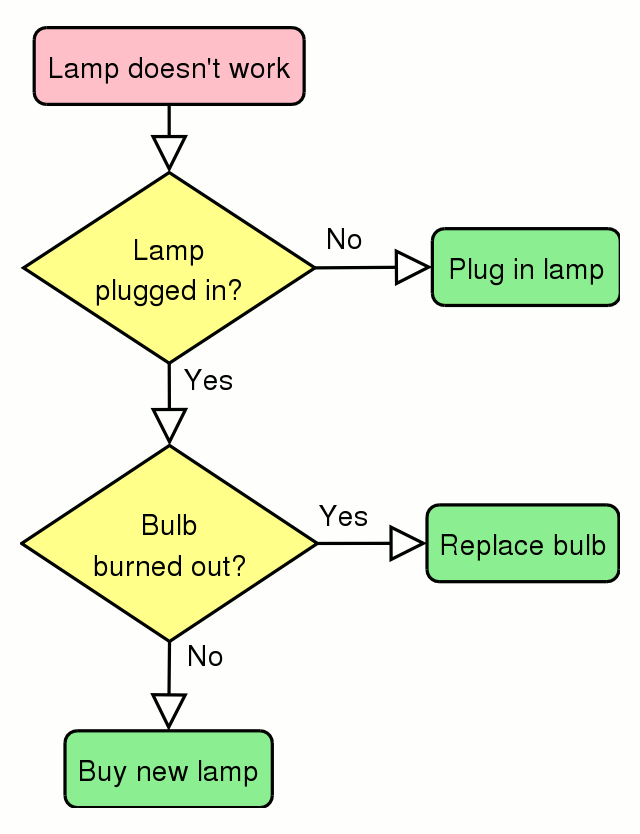
\includegraphics[width=.4\textwidth]{LampFlowchart}\\ % PNG-File
%  \caption{Nulla interdum aliquam leo}\label{fig:LampFlowchart}
%\end{figure}

%VERWEISE AUF ABBILDUNGEN:
%\ref{fig:LampFlowchart}
%\ref{fig:tabelle}

%Grafik aus PDF-File - diese Variante ist vorzuziehen, da sie die Einbundung echter Vektorgrafiken ermöglicht 
%\begin{figure}[htb]
%  \centering
%  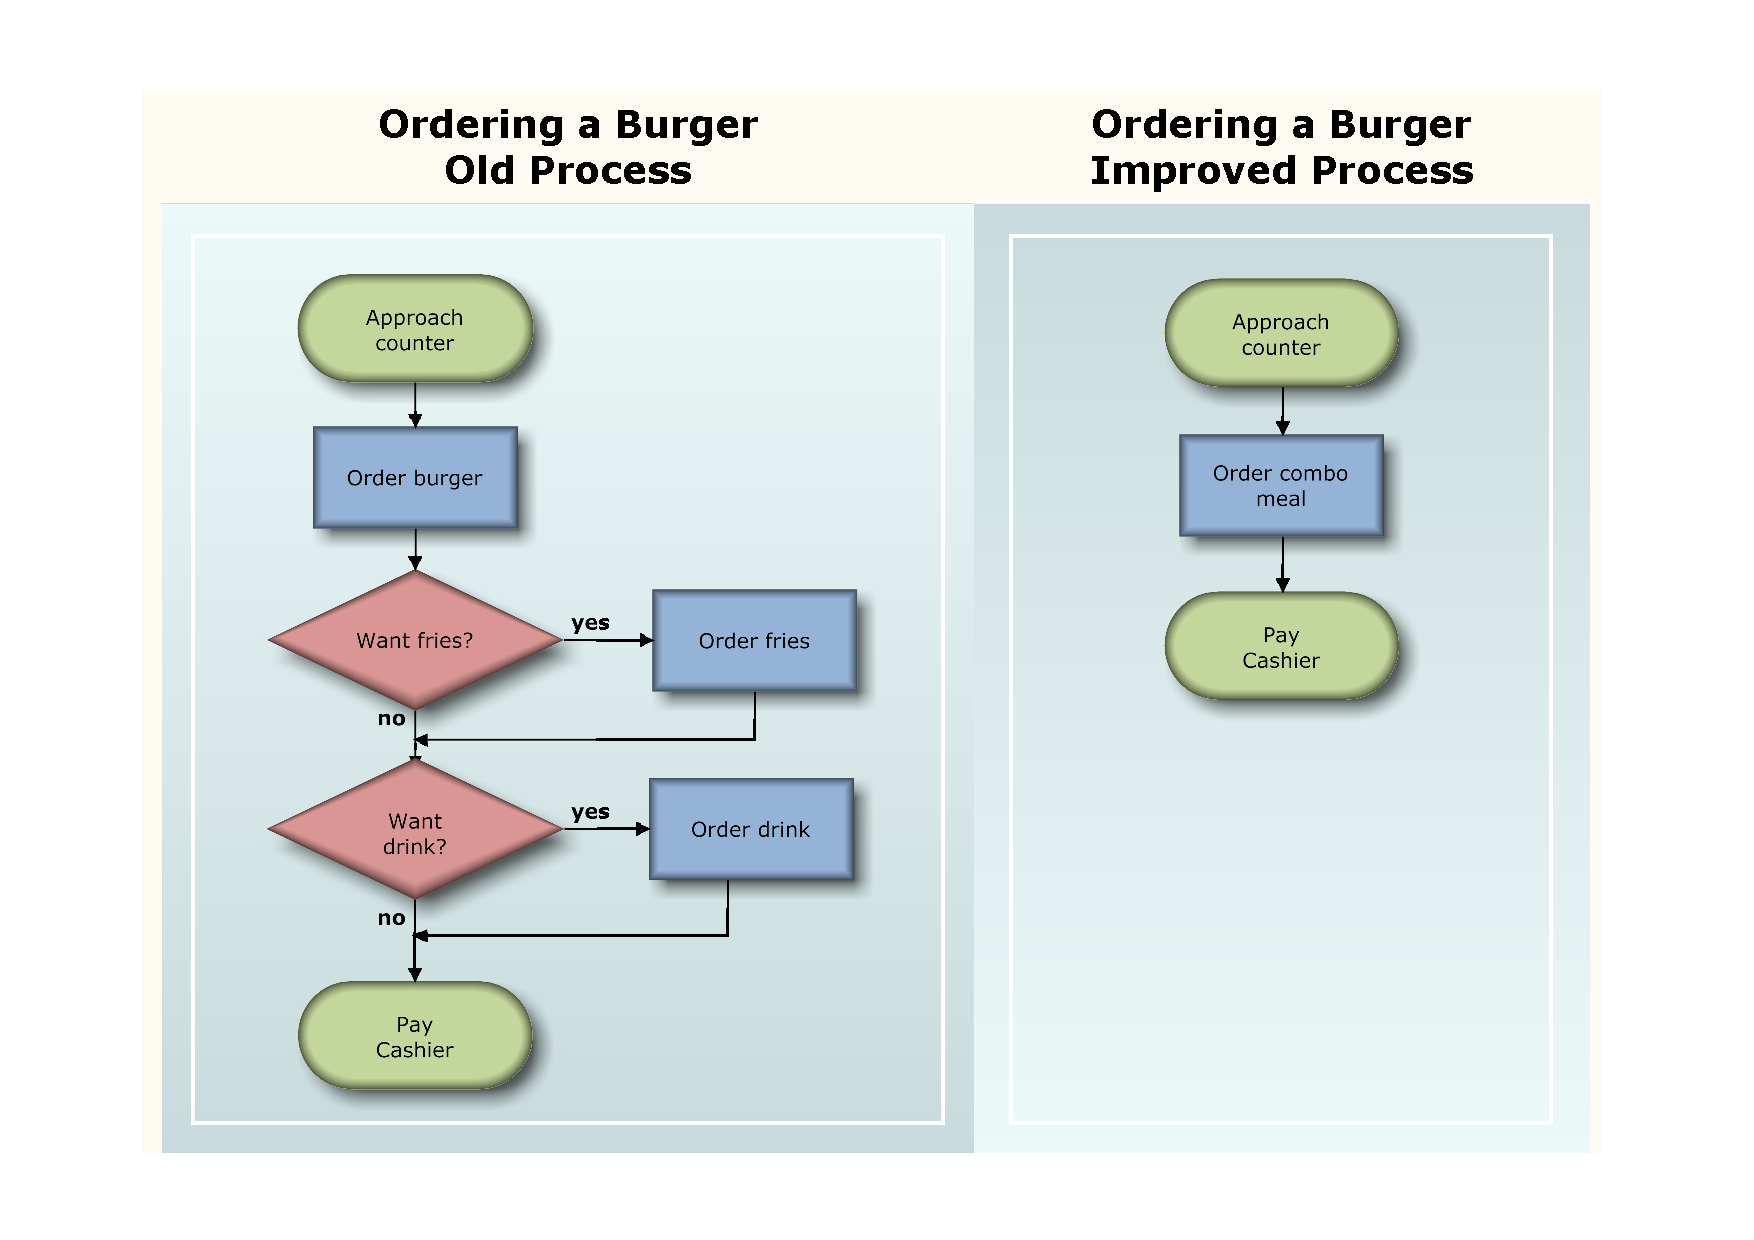
\includegraphics[scale=.6]{BurgerFlowchart}\\ % PDF-File
%  \caption{Donec tempor leo a massa \cite{scrguide07}}\label{fig:BurgerFlowchart}
%\end{figure}

%Tabellen im Regelfall auch in eine Figure-Umgebung setzen - Verwendung von Table-Umgebung lohnt nur bei sehr vielen Tabellen
%\begin{figure}[htb]
%  \centering
%  \begin{tabular}{|l|c|}
%    \hline
%    \textbf{tempus} & \textbf{risus} \\ \hline
%    ultrices & pellentesque \\
%    rhoncus & egestas \\
%    \hline
%  \end{tabular}
%  \caption{Aliquam fermentum}\label{fig:tabelle}
%\end{figure}



